% ============================================================
% 3a  NRG for two impurities
% ============================================================
\begin{frame}[t]
\ft{NRG for two impurities: even and odd channels}
\begin{columns}[T]
\begin{column}{0.50\textwidth}
\centering
\onslide<1->{\begin{tikzpicture}[x=1.0cm,y=0.95cm,font=\scriptsize]
 % host line and midpoint tick
 \draw[mygray] (-2.7,0) -- (2.7,0);
 \draw[mygray] (0,-0.12) -- (0,0.12);
 % dotted guides through the two impurity positions
 \foreach \x in {-1.3,1.3}{\draw[mygray,dotted] (\x,-1.75) -- (\x,1.6);}
 % even wave (same sign at both impurities), above the line
 \draw[verdigris,thick,domain=-2.2:2.2,samples=80,smooth,variable=\x] plot ({\x},{0.9-0.45*cos((\x*pi/1.3) r)});
 \node[verdigris,anchor=west] at (2.3,0.9) {even};
 % odd wave (opposite sign), below the line
 \draw[citron!70!black,thick,domain=-2.2:2.2,samples=80,smooth,variable=\x] plot ({\x},{-1.1+0.45*sin((\x*pi/2.6) r)});
 \node[citron!70!black,anchor=west] at (2.3,-1.1) {odd};
 % the two impurities (as in the RKKY cartoon, last step)
 \foreach \x in {-1.3,1.3}{\draw[cLM,fill=cLM!15,thick] (\x,0) circle (0.28);}
 \draw[->,cLM,>=stealth,line width=2.2pt] (-1.3,-0.3) -- (-1.3,0.45);
 \draw[->,cLM,>=stealth,line width=2.2pt] (1.3,0.3) -- (1.3,-0.45);
 % site labels
 \node[mygraydark,anchor=east] at (-1.62,-0.02) {$\vec r_1$}; \node[mygraydark,anchor=west] at (1.62,-0.02) {$\vec r_2$};
\end{tikzpicture}}

\vspace{0.25cm}
\onslide<2->{\begin{tikzpicture}[x=1.2cm,y=1.1cm,font=\scriptsize]
 % box with the two impurities
 \draw[mygray,rounded corners=4pt] (-0.1,-0.95) rectangle (1.0,0.95);
 \foreach \y in {0.4,-0.4}{\draw[cLM,fill=cLM!15,thick] (0.45,\y) circle (0.2);}
 \draw[->,cLM,>=stealth,line width=1.6pt] (0.45,0.25) -- (0.45,0.58);
 \draw[->,cLM,>=stealth,line width=1.6pt] (0.45,-0.25) -- (0.45,-0.58);
 % even chain: hoppings and sites shrink to the right
 \foreach \c/\y in {verdigris/0.5,citron!70!black/-0.5}{
  \draw[\c,line width=1.4pt] (1.0,\y*0.8) -- (1.4,\y);
  \foreach \a/\b/\w in {1.4/2.0/1.2,2.0/2.5/1.0,2.5/2.9/0.8,2.9/3.25/0.65,3.25/3.55/0.5}{\draw[\c,line width=\w pt] (\a,\y) -- (\b,\y);}
  \foreach \x/\r in {1.4/0.13,2.0/0.11,2.5/0.095,2.9/0.08,3.25/0.065,3.55/0.055}{\fill[\c] (\x,\y) circle (\r);}
  \foreach \x in {3.75,3.85,3.95}{\fill[\c] (\x,\y) circle (0.025);}}
 \node[verdigris,anchor=west] at (4.1,0.5) {even};
 \node[citron!70!black,anchor=west] at (4.1,-0.5) {odd};
 % energy arrow
 \draw[->,mygray,>=stealth] (1.4,-1.15) -- (3.9,-1.15);
 \node[mygraydark,anchor=north] at (2.65,-1.15) {energy scale $\Lambda^{-n/2}\to 0$};
\end{tikzpicture}}
\end{column}
\begin{column}{0.48\textwidth}
\vspace{0.2cm}
\onslide<1->{\begin{itemize}
 \item Sort the host electrons by parity about the midpoint
\end{itemize}
\vspace{0.1cm}{\small\hspace{1.2em}\textcolor{verdigris}{even: $\psi_{\rm e}\propto\psi(\vec r_1)+\psi(\vec r_2)$}\\[1pt]
\hspace{1.2em}\textcolor{citron!70!black}{odd: \ $\psi_{\rm o}\propto\psi(\vec r_1)-\psi(\vec r_2)$}\\[1pt]
\hspace{1.2em}{\footnotesize\color{mygraydark}$\psi(\vec r_i)$: host electron at impurity site $i$}\par}}
\onslide<2->{\begin{itemize}
 \item Each channel: one Wilson chain.\\ NRG treats both spins at once
\end{itemize}}
\vspace{0.2cm}
\onslide<3->{\centering{\large $\rho_{\rm e/o}(\omega) = \rho(0,\omega) \pm \colorbox{orchid!30}{$\rho(\vec r,\omega)$}$}\\[3pt]
{\small local $\pm$ non-local density of states:\\ the only input from the host\par}}
\onslide<2->{\vspace{0.2cm}\par\raggedright{\tiny\color{mygray} Jayaprakash, Krishna-murthy, Wilkins, PRL 47, 737 (1981)\\
Jones, Varma, Wilkins, PRL 61, 125 (1988)\\
Affleck, Ludwig, PRL 68, 1046 (1992)\\
Affleck, Ludwig, Jones, PRB 52, 9528 (1995)\par}}
\end{column}
\end{columns}
\onslide<3->{\tk{The low-energy local and non-local DoS must be well resolved}}
\end{frame}
% Notes: The two impurities couple to the even and odd parity combinations of the conduction electrons (Jayaprakash, Krishna-murthy, Wilkins; Jones, Varma): the sum and the difference of the host electron at the two impurity sites.
% Notes: Each channel is a Wilson chain; NRG solves both impurities at once. RKKY is not put in by hand (direct exchange is zero): it is generated together with Kondo.
% Notes: The channel densities of states are local plus/minus non-local: rho_e/o = rho(0,w) +/- rho(r,w). This is the only input from the host.
% Notes: NRG discretises energy logarithmically, so the input must be right on every scale, down to far below the meV van Hove singularity.

% ============================================================
% 3b  The DoS on every energy scale
% ============================================================
\begin{frame}[t]
\ft{The DoS on every energy scale}
\centering
\begin{tikzpicture}[font=\small]
 \path (0,1.25); % room under the title rule
 % momentum space: the Green's function is immediate from the band Hamiltonian
 \node[anchor=west,inner sep=2pt] (gk) at (0,0) {$G(\vec k,\omega)=\big[\omega+i\delta-H(\vec k)\big]^{-1}$};
 \node[anchor=north,font=\scriptsize,mygraydark] at (gk.south |- 0,-0.5) {momentum space: immediate from $H(\vec k)$};
 % real space: what a local impurity needs
 \node[anchor=west,inner sep=2pt] (gr) at (6.45,0) {$G(\vec r,\omega)=\displaystyle\int_{\rm BZ}\!\frac{d^2k}{(2\pi)^2}\;e^{i\vec k\cdot\vec r}\,G(\vec k,\omega)$};
 \node[anchor=north,font=\scriptsize,mygraydark] at (gr.south |- 0,-0.5) {real space: a 2D integral at every energy};
 \draw[->,>=stealth,thick,mygraydark] (gk.east) -- node[above,font=\scriptsize,align=center]{the impurity\\ is local} (gr.west);
\end{tikzpicture}\par
\vspace{-0.2cm}
\begin{columns}[T]
\begin{column}{0.54\textwidth}
\centering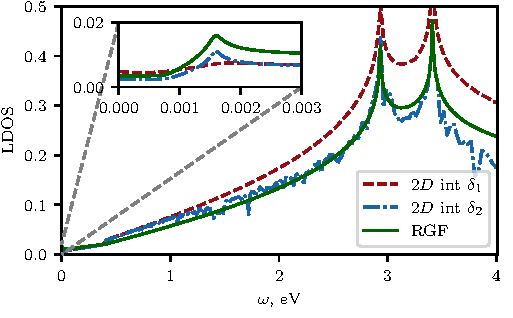
\includegraphics[width=\linewidth]{figures/fig2_blg_ldos_comparison.pdf}
{\tiny\color{mygray} LDoS on an unstacked site (A1/B2). $\delta_{1,2}$: two broadenings of the 2D integral\par}
\end{column}
\begin{column}{0.42\textwidth}
\vspace{0.6cm}
NRG: logarithmic energy grid,\\ down to \colorbox{citron!40}{\mystrut far below 1 meV}\par
\vspace{0.45cm}
van Hove peak:\\ $\sim 10^{-4}$ of the Brillouin zone\par
\vspace{0.45cm}
Recursive Green's functions (RGF):\\ smooth, peak resolved\par
\end{column}
\end{columns}
\onslide<2->{\tk{Direct integration is noisy: unsuitable for the logarithmic grid of NRG}}
\end{frame}
% Notes: Why an integral at all: in momentum space G(k) is just the inverse of omega - H(k). But the impurity sits on one site, so we need G in real space: a Fourier transform, i.e. a 2D Brillouin-zone integral, at every energy. Its imaginary part is the local (r = 0) or non-local DoS.
% Notes: The inset is the meV window around the van Hove peak at 1.6 meV, which occupies about 1e-4 of the Brillouin zone.
% Notes: Direct 2D integration: the broad broadening smears the van Hove peak; the small broadening is noisy at all energies.
% Notes: Recursion with an adaptive broadening (1e-5 below 0.2 meV, 0.05|omega| up to 20 meV, 1e-3 above) is smooth and resolves the peak: next slide.

% ============================================================
% 3c  Fast recursive Green's functions
% ============================================================
\begin{frame}[t]
\ft{Fast recursive Green's functions}
\begin{columns}[T]
\begin{column}{0.43\textwidth}
\vspace{0.2cm}
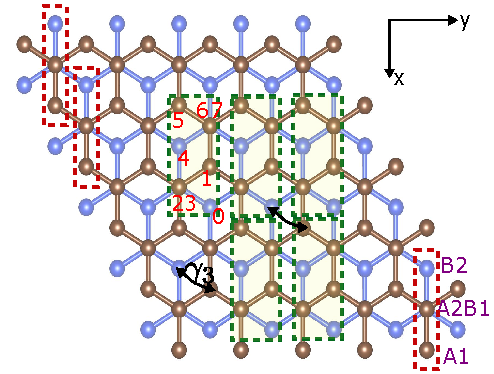
\includegraphics[width=\linewidth]{figures/BLG_regv2.pdf}
{\tiny\color{mygray} Bilayer graphene redrawn as a square lattice of 8-site cells\par}
\vspace{0.15cm}
\centering
\begin{tikzpicture}[x=0.6cm,y=0.56cm,font=\scriptsize]
 % effective square lattice of 8-site cells (y to the right, x downwards, as in the figure above)
 \foreach \j in {0,1,2}{\draw[mygray,line width=0.6pt] (-0.35,-\j) -- (5.35,-\j);}
 \foreach \i in {0,...,5}{\draw[mygray,line width=0.6pt] (\i,0.35) -- (\i,-2.35);}
 \foreach \i in {0,...,5}{\foreach \j in {0,1,2}{\draw[mygraydark,dashed,fill=citron!25] (\i-0.3,-\j-0.3) rectangle (\i+0.3,-\j+0.3);}}
 % y: the direction of the fast recursion
 \draw[->,>=stealth,line width=1.0pt] (-0.3,-2.85) -- (5.3,-2.85);
 \node[anchor=north] at (2.5,-2.9) {$y$: fast recursion};
 % x: Fourier transform, then the adaptive k_x integral
 \draw[->,>=stealth,line width=1.0pt] (-0.9,0.3) -- (-0.9,-2.3);
 \node[rotate=90,anchor=south] at (-0.95,-1.0) {$x$: $k_x$ integral};
\end{tikzpicture}\par
\vspace{0.05cm}
\raggedright{\tiny\color{mygray} Cuba (Cuhre): Hahn, Comput. Phys. Commun. 168, 78 (2005)\\
Python interface: Buchner, github.com/JohannesBuchner/cuba\par}
\end{column}
\begin{column}{0.55\textwidth}
\vspace{0.2cm}
\onslide<1->{1. Fourier transform along $x$:\\ \hspace{1.1em}for each $k_x$, a 1D chain of cells along $y$\par
\vspace{0.15cm}
\hspace{1.1em}\begin{tikzpicture}[x=0.44cm,y=0.5cm,font=\scriptsize]
 % the chain: identical 8-site cells joined by the y hopping
 \draw[mygraydark,line width=1pt] (-0.9,0.27) -- (8.8,0.27);
 \foreach \i in {0,...,6}{\draw[mygraydark,dashed,fill=citron!25] (\i*1.3,0) rectangle (\i*1.3+0.9,0.55);}
 \node[mygraydark,anchor=east] at (-0.9,0.27) {$\cdots$}; \node[mygraydark,anchor=west] at (8.8,0.27) {$\cdots$};
 % one cell is the 8-site supercell
 \draw[mygraydark,decorate,decoration={brace,mirror,amplitude=2pt}] (3.9,-0.15) -- (4.8,-0.15);
 \node[mygraydark,anchor=north] at (4.35,-0.3) {8 sites};
 \node[mygraydark,anchor=west] at (9.9,0.27) {$y\,\rightarrow$};
\end{tikzpicture}\par}
\vspace{0.2cm}
\onslide<2->{2. Recursion: each step doubles the chain\par
\vspace{0.15cm}
\hspace{1.1em}\begin{tikzpicture}[x=0.44cm,y=0.5cm,font=\footnotesize]
 % chains of 1, 2, 4, 8 cells: each stage joins two copies of the previous one
 \foreach \n/\y in {1/3,2/2,4/1,8/0}{
  \draw[mygraydark,line width=1pt] (0.45,\y*0.85+0.27) -- ({(\n-1)*1.3+0.45},\y*0.85+0.27);
  \foreach \i in {1,...,\n}{\draw[mygraydark,dashed,fill=citron!25] ({(\i-1)*1.3},\y*0.85) rectangle ({(\i-1)*1.3+0.9},\y*0.85+0.55);}
  \node[mygraydark,anchor=west] at (10.6,\y*0.85+0.27) {\n};}
 \node[mygraydark] at (0.45,-0.55) {$\vdots$};
 \node[mygraydark,anchor=west] at (1.2,-0.6) {$N$ steps: $2^N$ cells, only $8\times 8$ matrices};
\end{tikzpicture}\par}
\vspace{0.2cm}
\onslide<3->{3. Adaptive integral over $k_x$ (Cuhre):\par
\vspace{0.05cm}
\centering{\small $G(\vec r,\omega)=\int\!\frac{dk_x}{2\pi}\,e^{ik_x x}\,G_{\rm chain}(k_x,\omega)$\\[4pt] $\Rightarrow$\ \ \colorbox{orchid!30}{\mystrut $\rho(0,\omega),\ \rho(\vec r,\omega)$}}\par}
\vspace{0.2cm}
\raggedright{\tiny\color{mygray} L\'opez Sancho, L\'opez Sancho, Rubio, J. Phys. F: Met. Phys. 14, 1205 (1984)\\
Lewenkopf, Mucciolo, J. Comput. Electron. 12, 203 (2013)\par}
\end{column}
\end{columns}
\end{frame}
% Notes: Redraw BLG as a square lattice of 8-site cells (left). Fourier transform along x: for each k_x what is left is a 1D chain of cells along y.
% Notes: The recursion is the Lopez Sancho quick iterative scheme; our code is built on it.
% Notes: Each step is only 8x8 matrix algebra and doubles the length, so 2^N cells cost N steps.
% Notes: The remaining k_x integral is done with an adaptive cubature: the Cuhre routine of the Cuba library (Hahn), through Buchner's Python interface.
% Notes: Output: the local and non-local Green's function at any energy, with broadening as small as needed.

% ============================================================
% 4  BLG sites
% ============================================================
\begin{frame}
\ft{Bernal bilayer: stacked and unstacked sites see very different DoS}
\begin{columns}[T]
\begin{column}{0.36\textwidth}
\centering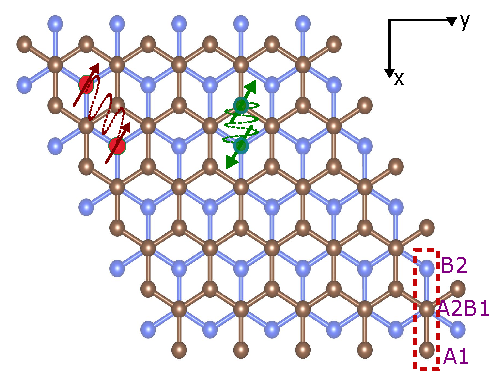
\includegraphics[width=\linewidth]{figures/BLG_regv3.pdf}
\vspace{0.1cm}\par
\sitemap[0.85]{0}\\[2pt]\legend{0}
\end{column}
\begin{column}{0.62\textwidth}
\centering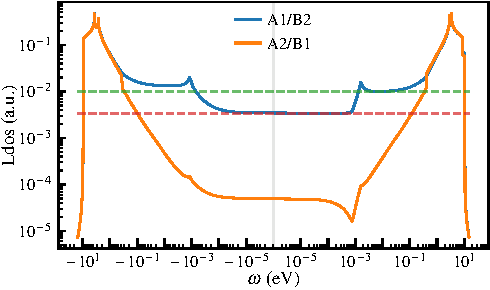
\includegraphics[width=0.92\linewidth]{figures/ldos.pdf}
\begin{itemize}\small
 \item A1/B2 (unstacked): large LDoS, trigonal-warping vHs at $\sim$1.6 meV
 \item A2/B1 (stacked): suppressed LDoS at low energy
\end{itemize}
\end{column}
\end{columns}
\tk{Same lattice, two kinds of site: what does an impurity feel?}
\end{frame}
% Notes: - Bernal BLG: B1 sits on A2 (stacked, dimer), A1 and B2 have no site above/below (unstacked).
% - LDoS: A1/B2 enhanced with a vHs at ~1.6 meV from trigonal warping; A2/B1 strongly suppressed at low energy.
% - Site map (bottom left) is empty now: we will colour it by physics as results arrive.
